% Q3 (Ti/Tv) next to its oracle, for the main text's validation paragraph.
% Sources verified against VCF-RDFizer v3.3.1 (identical at v3.1.0):
%   src/validation/queries/common/q03_titv.rq            (the query, abridged here)
%   src/validation/validation_runner.py: TRANSITIONS, alt_lexical(),
%       parse_vcf() lines 1572-1576 (the counters), 1816-1820 (the summary),
%       normalize()/compare() (exact comparison; Ti/Tv derived from the counts).
% Abridged: the PREFIX line is dropped, and the query's four-way transition test
% (A>G, G>A, C>T, T>C) is written as isTransition(); the oracle is pseudo-code.
% Build: pdflatex -interaction=nonstopmode -halt-on-error fig-query-oracle.tex
\documentclass[border=3pt]{standalone}
\usepackage[T1]{fontenc}
\usepackage{lmodern}
\usepackage{helvet}
\renewcommand{\familydefault}{\sfdefault}
\usepackage{listings}
\usepackage{tikz}
\usetikzlibrary{arrows.meta,calc,positioning}
\definecolor{teal}{HTML}{1F7F83}
\definecolor{tealbg}{HTML}{E8F3F2}
\definecolor{gold}{HTML}{A37B17}
\definecolor{goldbg}{HTML}{FBF2DB}
\definecolor{ink}{HTML}{26343D}
\definecolor{muted}{HTML}{5C6770}
\definecolor{light}{HTML}{F3F5F6}
\lstset{basicstyle=\ttfamily\fontsize{6.6}{8.1}\selectfont\color{ink}, columns=fullflexible,
  keepspaces=true, showstringspaces=false, upquote=true, aboveskip=0pt, belowskip=0pt,
  keywordstyle=\bfseries}
\lstdefinelanguage{sparqlq}{morekeywords={SELECT,WHERE,BIND,FILTER,COUNT,DISTINCT,SUM,IF,AS,REGEX,UCASE,STR,a},
  sensitive=true, morestring=[b]"}
\lstdefinelanguage{pseudo}{morekeywords={for,in,if,else,and,not},
  sensitive=true, morestring=[b]"}
\newsavebox{\sparqlbox}
\newsavebox{\oraclebox}
\begin{document}
\begin{lrbox}{\sparqlbox}\begin{minipage}{6.55cm}
\begin{lstlisting}[language=sparqlq]
SELECT
  (COUNT(DISTINCT ?record) AS ?biallelicSnvCount)
  (SUM(IF(isTransition(?ref, ?alt), 1, 0))
                           AS ?transitionCount)
  (SUM(IF(isTransition(?ref, ?alt), 0, 1))
                           AS ?transversionCount)
WHERE {
  ?record a vcfc:VCFRecord ;
          vcfc:ref ?refLiteral ;
          vcfc:alt ?altLiteral .
  BIND(UCASE(STR(?refLiteral)) AS ?ref)
  BIND(UCASE(STR(?altLiteral)) AS ?alt)
  FILTER(REGEX(?ref, "^[ACGT]$") &&
         REGEX(?alt, "^[ACGT]$") && ?ref != ?alt)
}
\end{lstlisting}
\end{minipage}\end{lrbox}
\begin{lrbox}{\oraclebox}\begin{minipage}{6.55cm}
\begin{lstlisting}[language=pseudo]
TRANSITIONS = {(A,G), (G,A), (C,T), (T,C)}
snvs = transitions = transversions = 0

for record in cyvcf2.VCF(source_vcf):
    ref = upper(record.REF)
    alt = upper(join(record.ALT, ","))
    if ref in {A,C,G,T} and alt in {A,C,G,T}
            and ref != alt:
        snvs += 1
        if (ref, alt) in TRANSITIONS:
            transitions += 1
        else:
            transversions += 1

expected = {biallelicSnvCount: snvs,
            transitionCount: transitions,
            transversionCount: transversions}
\end{lstlisting}
\end{minipage}\end{lrbox}
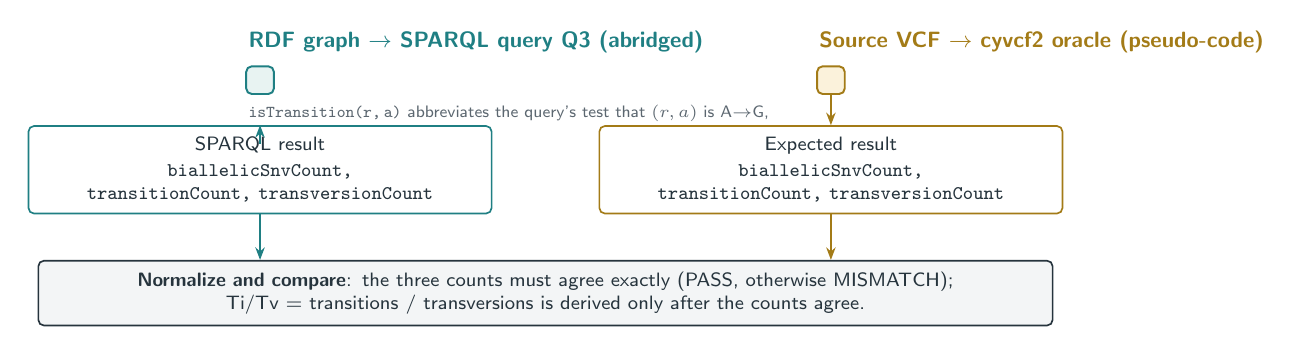
\begin{tikzpicture}[
  x=1cm,y=-1cm,
  font=\fontsize{7.6}{9}\selectfont, text=ink,
  code/.style={rounded corners=2pt,line width=.7pt,inner sep=5pt,anchor=north west},
  head/.style={anchor=south west,inner sep=1pt,font=\fontsize{8}{9.4}\selectfont\bfseries},
  result/.style={rounded corners=2pt,line width=.6pt,inner sep=4pt,align=center,font=\fontsize{7}{8.4}\selectfont},
  flow/.style={-{Stealth[length=4.5pt]},line width=.8pt},
]
% Headers and code panels
\node[head,text=teal] at (0,0) {RDF graph \(\rightarrow\) SPARQL query Q3 (abridged)};
\node[head,text=gold] at (7.25,0) {Source VCF \(\rightarrow\) cyvcf2 oracle (pseudo-code)};
\node[code,draw=teal,fill=tealbg] (q) at (0,0.12) {\usebox{\sparqlbox}};
\node[code,draw=gold,fill=goldbg] (o) at (7.25,0.12) {\usebox{\oraclebox}};
\node[anchor=north west,inner sep=1pt,text=muted,font=\fontsize{6.4}{7.6}\selectfont,text width=6.7cm]
  at ($(q.south west)+(0,0.08)$) {\texttt{isTransition(r,\,a)} abbreviates the query's test that \((r,a)\) is A\(\rightarrow\)G, G\(\rightarrow\)A, C\(\rightarrow\)T, or T\(\rightarrow\)C.};
% Results and comparison: both result boxes sit below the taller (oracle) panel
\path (q.south |- o.south) ++(0,0.95) node[result,draw=teal,fill=white,text width=5.6cm] (qr)
  {SPARQL result\\[1pt]\texttt{biallelicSnvCount, transitionCount, transversionCount}};
\path (o.south) ++(0,0.95) node[result,draw=gold,fill=white,text width=5.6cm] (or)
  {Expected result\\[1pt]\texttt{biallelicSnvCount, transitionCount, transversionCount}};
\draw[flow,draw=teal] ($(q.south)+(0,0.62)$) -- (qr.north);
\draw[flow,draw=gold] (o.south) -- (or.north);
\path ($(qr.south)!0.5!(or.south)$) ++(0,1.0) node[result,draw=ink,fill=light,text width=12.6cm] (cmp)
  {\textbf{Normalize and compare}: the three counts must agree exactly (PASS, otherwise \mbox{MISMATCH});\\
   Ti/Tv \(=\) transitions \(/\) transversions is derived only after the counts agree.};
\draw[flow,draw=teal] (qr.south) -- (qr.south |- cmp.north);
\draw[flow,draw=gold] (or.south) -- (or.south |- cmp.north);
\end{tikzpicture}
\end{document}
